% Network schematic for the fractional-flow routing example
% (CHEME-153-M2-FractionalFlowRouting-MWA-Ungraded-Codio.ipynb)
%
% Link--route incidence (rows = links, cols = routes P1..P4), capacities b:
%   e0 trunk     [1 1 1 1]   cap 12   (all routes; the bottleneck = max flow)
%   eL sub-trunk [1 1 0 0]   cap  5   (routes 1,2)
%   e1 branch    [1 0 0 0]   cap  2   (route 1; tightest)
%   e2 branch    [0 1 0 0]   cap  6   (route 2)
%   e3 branch    [0 0 1 0]   cap  6   (route 3)
%   e4 branch    [0 0 0 1]   cap  6   (route 4)
%
% Routes:  P1: e0->eL->e1   P2: e0->eL->e2   P3: e0->e3   P4: e0->e4
%
% Build:  pdflatex flow-routing.tex
\documentclass[border=10pt]{standalone}
\usepackage{amsmath}
\usepackage{tikz}
\usetikzlibrary{arrows.meta, positioning, calc, backgrounds}

\begin{document}
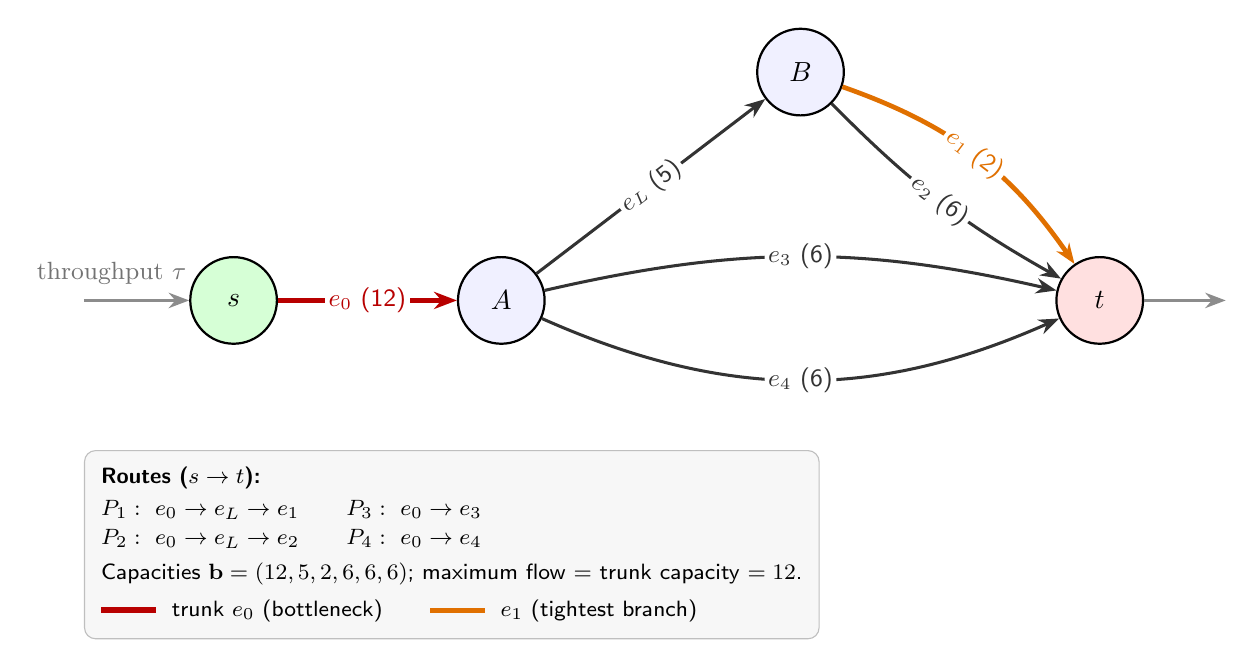
\begin{tikzpicture}[
    >={Stealth[length=2.6mm, width=2.2mm]},
    font=\sffamily,
    nd/.style     = {circle, draw=black, line width=0.8pt, minimum size=11mm, inner sep=0pt, fill=blue!6},
    source/.style = {nd, fill=green!16},
    sink/.style   = {nd, fill=red!12},
    flow/.style   = {-{Stealth[length=2.6mm]}, line width=1.1pt, black!80},
    trunk/.style  = {-{Stealth[length=2.9mm]}, line width=2.1pt, red!72!black},
    tight/.style  = {-{Stealth[length=2.6mm]}, line width=1.7pt, orange!88!black},
    clab/.style   = {font=\small\sffamily, fill=white, inner sep=1.3pt, rounded corners=1pt},
    inout/.style  = {-{Stealth[length=2.6mm]}, line width=1.1pt, black!45}
  ]

  % --- nodes ---
  \node[source] (s) at (0,0)     {$s$};
  \node[nd]     (A) at (3.4,0)   {$A$};
  \node[nd]     (B) at (7.2,2.9) {$B$};
  \node[sink]   (t) at (11.0,0)  {$t$};

  % --- injected throughput tau and drained flow ---
  \draw[inout] ($(s)+(-1.9,0)$) -- (s);
  \node[font=\small, black!55] at (-1.55,0.34) {throughput $\tau$};
  \draw[inout] (t) -- ($(t)+(1.6,0)$);

  % --- links ---
  \draw[trunk] (s) -- node[clab]{$e_0$ (12)} (A);
  \draw[flow]  (A) -- node[clab, sloped]{$e_L$ (5)} (B);

  \draw[tight] (B) to[bend left=18]  node[clab, sloped]{$e_1$ (2)} (t);
  \draw[flow]  (B) to[bend right=8]  node[clab, sloped]{$e_2$ (6)} (t);

  \draw[flow]  (A) to[bend left=13]  node[clab]{$e_3$ (6)} (t);
  \draw[flow]  (A) to[bend right=24] node[clab]{$e_4$ (6)} (t);

  % --- legend (single box: routes, capacities, and the colour key) ---
  \node[anchor=north west, align=left, draw=black!25, rounded corners,
        fill=black!3, inner sep=6pt, font=\footnotesize\sffamily] at (-1.9,-1.9)
    {\textbf{Routes ($s \to t$):}\\[2pt]
     $P_1:\ e_0 \to e_L \to e_1$\qquad $P_3:\ e_0 \to e_3$\\[1pt]
     $P_2:\ e_0 \to e_L \to e_2$\qquad $P_4:\ e_0 \to e_4$\\[3pt]
     Capacities $\mathbf{b}=(12,5,2,6,6,6)$; maximum flow $=$ trunk capacity $= 12$.\\[4pt]
     \textcolor{red!72!black}{\rule[0.35ex]{7mm}{2.1pt}}~~trunk $e_0$ (bottleneck)\qquad
     \textcolor{orange!88!black}{\rule[0.35ex]{7mm}{1.7pt}}~~$e_1$ (tightest branch)};

\end{tikzpicture}
\end{document}
